\documentclass[UTF8]{article}
\usepackage{ctex}
\usepackage{anyfontsize}
\usepackage{bookmark}
\hypersetup{hidelinks}
\usepackage{tikz}
\usepackage{pgfplots}
\pgfplotsset{compat=1.5}
\usepackage{tocbibind}
\usepackage{geometry}
\usepackage{amsmath}
\numberwithin{equation}{section}
\usepackage{mathrsfs}
% \usepackage{newpxmath}
\usepackage{physics}
\usepackage{booktabs}
\usepackage{esint} 
\geometry{a4paper,scale=0.8}

\title{普通物理}
\author{李承高}
\begin{document}
\maketitle
\thispagestyle{empty}
\newpage
\thispagestyle{empty}
\tableofcontents
\newpage

\pagenumbering{arabic}

\section{牛顿力学}
\subsection{多粒子系统}
在牛顿力学体系中,我们采用质点系来描述。质心运动定理:整个系统的受力可以看成
全部的质量集中于质心,然后只收外力的作用,内力相互抵消了:
\begin{align*}
    a=\frac{d^2r_c}{dt^2}=\frac{\sum_i m_i a_i}{\sum_i m_i}
\end{align*}
质点系的动能定理:
\begin{align*}
    \int F_1 dr_1+\int F_2 dr_2+\int F_{12}dr_1+\int F_{21}dr_2=\Delta E_{k1}+\Delta E_{k2}
\end{align*}
也可以写成:
\begin{align*}
    A_e+A_i=\Delta E_k
\end{align*}
前一项是外力做功,后面一项是内力做功,注意到前面分析受力时,内力是约掉的,但是涉及
到积分之后,不能直接约掉了,内力做功又可分为保守内力做的功,和非保守内力做的功。保守
内力做的功可以转化到系统势能的改变,因此从状态1到状态2的变化中,机械能的增量等于外力
做的功和非保守内力做功的总和。注意:保守力是对系统而言的,也就是说内力分为保守力
和非保守力才是有意义的,质点系的功能原理:
\begin{align*}
    A_e+A_{in}=\Delta E
\end{align*}
\subsection{转动动力学}
刚性物体:体积不发生改变的物体

转动惯量的计算(重要):
\begin{align*}
    I=\sum_i m_ir_i^2=\int r^2\rho dr
\end{align*}
平行轴定理:
\begin{align*}
    I_n=I_{cm}+md^2
\end{align*}

由N个物质组成的一般系统的定能:
\begin{align*}
    K=\frac{1}{2}mv^2+K_{cm}
\end{align*}
第一项为质心的动能,第二项为质心系中的质点的动能。

平动加转动:
对于圆盘的无滑滚动:
\begin{align*}
    &v=\omega R\\
    &K=\frac{1}{2}m(\omega R)^2+\frac{1}{2}I\omega^2\\
    &K=\frac{1}{2}(\frac{3}{2}mR^2)\omega^2
\end{align*}
由平行轴定理可以得到:
\begin{align*}
    I=I_{cm}+md^2
\end{align*}
则可以将无滑滚动看成绕圆周上一点的转动。一般来说,平动的动能和转动的动能无关,但是对于无滑滚动
情况,他们是相互关联的。

复杂转动:定滑轮下面用轻绳连接一个木块。轻绳保证了绳子两端的拉力相等,这里注意不是
轻滑轮,因此需要考虑转动惯量,采用两种观点来分析,牛顿力学受力分析或者能量观点来分析
,能量观点在各个地方都是特别重要的。

角动量守恒:一根杆上有两个圆盘,上面的角速度为$\omega$,下面的角速度为0,上面的圆盘
落下来之后一起转动,类似于完全非弹性碰撞:
\begin{align*}
    I_1\omega = (I_1+I_2)\omega'
\end{align*}

非刚性物体在不受外力矩情况下的角动量守恒:对于转动的人:
\begin{align*}
    &I_1\omega_1=I_2\omega_2\\
    &\frac{1}{2}I_1\omega_1^2\neq \frac{1}{2}I_2\omega_2^2
\end{align*}
动能的改变来源于肌肉的径向运动做功。

静平衡条件:对于一个受外力矩的物体,静平衡的条件有:
\begin{align*}
    \sum_iF_i=0\\
    \sum_i \tau_i=0
\end{align*}
计算力矩和时,选取的转轴所在的点的外力不方便求时最好,这样由于r=0使得这个力尽管
不知道也是没事的。

悬挂指示牌:
\begin{center}
\tikzset{every picture/.style={line width=0.75pt}} %set default line width to 0.75pt        
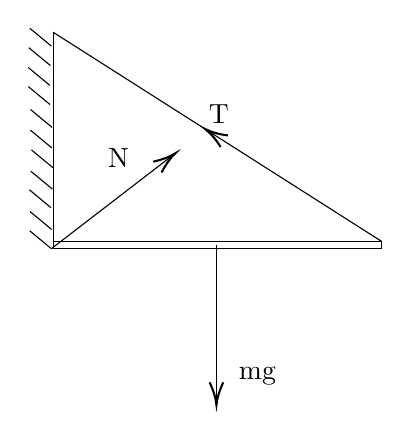
\begin{tikzpicture}[x=0.75pt,y=0.75pt,yscale=-1,xscale=1]
%uncomment if require: \path (0,300); %set diagram left start at 0, and has height of 300

%Straight Lines [id:da806382422982244] 
\draw    (240,50.37) -- (240,154.64) ;
%Straight Lines [id:da31871242929214283] 
\draw    (228.72,48.42) -- (239.12,57.04) ;
%Straight Lines [id:da4416675488053512] 
\draw    (228.25,57.79) -- (238.65,66.41) ;
%Straight Lines [id:da4135647161625422] 
\draw    (227.97,67.33) -- (238.37,75.95) ;
%Straight Lines [id:da3303180096005154] 
\draw    (228.03,76.56) -- (238.44,85.18) ;
%Straight Lines [id:da993303032173324] 
\draw    (229.07,87.58) -- (239.47,96.2) ;
%Straight Lines [id:da2083713559280047] 
\draw    (228.97,97.48) -- (239.37,106.1) ;
%Straight Lines [id:da12955295024730806] 
\draw    (229.53,107.05) -- (239.94,115.67) ;
%Straight Lines [id:da08375799704767561] 
\draw    (229.2,117.29) -- (239.6,125.91) ;
%Straight Lines [id:da6402333489332137] 
\draw    (228.53,126.27) -- (238.94,134.89) ;
%Straight Lines [id:da021151268849388005] 
\draw    (228.83,136.73) -- (239.24,145.35) ;
%Straight Lines [id:da5725193266344872] 
\draw    (228.7,146.02) -- (239.11,154.64) ;
%Flowchart: Process [id:dp11550730951992527] 
\draw   (240,151.1) -- (398.2,151.1) -- (398.2,154.64) -- (240,154.64) -- cycle ;
%Straight Lines [id:da9392381307860376] 
\draw    (318.65,152.87) -- (318.65,227.98) ;
\draw [shift={(318.65,229.98)}, rotate = 270] [color={rgb, 255:red, 0; green, 0; blue, 0 }  ][line width=0.75]    (10.93,-3.29) .. controls (6.95,-1.4) and (3.31,-0.3) .. (0,0) .. controls (3.31,0.3) and (6.95,1.4) .. (10.93,3.29)   ;
%Straight Lines [id:da8133358051249739] 
\draw    (239.11,154.64) -- (297.31,109.86) ;
\draw [shift={(298.89,108.64)}, rotate = 142.43] [color={rgb, 255:red, 0; green, 0; blue, 0 }  ][line width=0.75]    (10.93,-3.29) .. controls (6.95,-1.4) and (3.31,-0.3) .. (0,0) .. controls (3.31,0.3) and (6.95,1.4) .. (10.93,3.29)   ;
%Straight Lines [id:da9743703423144661] 
\draw    (240,50.37) -- (398.2,151.1) ;
\draw [shift={(313.2,96.97)}, rotate = 32.49] [color={rgb, 255:red, 0; green, 0; blue, 0 }  ][line width=0.75]    (10.93,-3.29) .. controls (6.95,-1.4) and (3.31,-0.3) .. (0,0) .. controls (3.31,0.3) and (6.95,1.4) .. (10.93,3.29)   ;


% Text Node
\draw (328.24,210.69) node [anchor=north west][inner sep=0.75pt]   [align=left] {mg};
% Text Node
\draw (265.18,104.92) node [anchor=north west][inner sep=0.75pt]   [align=left] {N};
% Text Node
\draw (313.72,83.99) node [anchor=north west][inner sep=0.75pt]   [align=left] {T};


\end{tikzpicture}
\end{center}
墙对杆的力不是垂直于墙的,列出静平衡方程:
\begin{align*}
    &T\sin \theta +P_y-mg=0\\
    &P_x-T\cos \theta = 0\\
    &Tr\sin \theta +mg\frac{L}{2}=0
\end{align*}

三维刚体动力学:
$\tau$,L的定义:
\begin{align*}
    \tau = r\times F\\
    L=r\times p
\end{align*}
\subsection{狭义相对论}
狭义相对论的两条基本公理:1.相对性原理(所有惯性参考系都是等价的)2. 光速不变原理
(若牛顿运动定律对你是成立的,那么你就是惯性系中的观察者)

在SR中,不能假设长度和时间对于所有的观察者都是相同的,这是和牛顿时空观下的伽利略
变换所不同的地方。对于一维情况下的洛伦兹变换的推导(逆变换的形式就是分子全部换成加号):
\begin{align*}
    &x=ct,x'=ct'\\
    &x=\gamma(x'+u t'),x'=\gamma(x-u t)\\
    &c^2tt' = \gamma^2 (c^2 tt'-u^2 tt')\\
    &\gamma^2 = \frac{1}{1-u^2/c^2}
\end{align*}
因此我们得到洛伦兹坐标变换关系:
\begin{align*}
    &x'=\frac{x-u t}{\sqrt{1-u^2/c^2}}\\
    &t'=\frac{t-(ux/c^2)}{\sqrt[]{1-u^2/c^2}}
\end{align*}
洛伦兹距离变换公式:
\begin{align*}
    &\Delta x'=\frac{\Delta x-u \Delta t}{\sqrt{1-u^2/c^2}}\\
    &\Delta t'=\frac{\Delta t-(u\Delta x/c^2)}{\sqrt[]{1-u^2/c^2}}
\end{align*}
洛伦兹速度变换公式(逆变换的形式就是减号全部变成加号):
\begin{align*}
    v'=\frac{\Delta x'}{\Delta t'}=\frac{v-u}{1-(uv/c^2)}
\end{align*}
洛伦兹变换的物理意义:$(x,t)\xrightarrow{transformation} (x',t')$,这是一个线性
映射:
\begin{align*}
    \mqty[x'\\t']=\mqty[\gamma&-u\gamma\\ -(u/c^2)\gamma&\gamma]\mqty[x\\t]
\end{align*}

同时的相对性:‘我看你的时间是变慢的,你看我的时间也是变慢的’,可以假设$x=0$,根据
洛伦兹变换得到:$t'>t$。利用洛伦兹逆变换,$x'=0$,得到:$t>t'$。

尺缩效应:测量运动的物体的长度会缩短,需要注意的是测量物体的长度必须是在相对于
物体静止的参考系下测量,并且需要同时测,因此通过洛伦兹逆变换把运动参考系下的长度变换到静止参考系
的长度公式:$\Delta x = \Delta x' \sqrt{1-(u^2/c^2)}$.

需要注意的是狭义相对论中的速度变换都是满足洛伦兹变换的,此时不能轻易的使用伽利略变换
,最重要的是选取坐标系,例如对于两个相对于地面相反运动的飞船,B飞船相对于A飞船的
速度为多少,这里采用的就是选取A飞船为运动参考系,地面为相对观察者静止的参考系,
A在地面参考系的速度已知,B参考系相对于地面参考系的速度已知,只需要使用洛伦兹速度变换
关系即可得到答案。\\
相对论动力学:
牛顿运动定律的普适形式:
\begin{align*}
    F=\frac{d(mv)}{dt}
\end{align*}
这个方程不满足SR的两条基本假设,SR力学基本方程:
\begin{align*}
    F=\frac{d}{dt}(\frac{m_0}{\sqrt{1-(v/c)^2}}v)
\end{align*}
质能关系:
\begin{align*}
    &Fdt=dp,Fds=dE_k\\
    &v=\frac{dE}{dp}\\
    &E=mc^2,E_0=m_0c^2\\
    &E_k=(m-m_0)c^2
\end{align*}
\section{热力学}
\subsection{理想气体}
平衡态:在没有外界干扰的孤立系统的宏观态不随时间的改变而改变。

准静态过程:当气体的外界条件发生改变时,气体的状态变化是十分缓慢的,每次状态的
变化都可以看成近似平衡的。

理想气体的物态方程:
\begin{align*}
    PV=\mu RT=\frac{N}{N_A}RT\\
    P=\frac{N}{V}\frac{R}{N_A}T=nkT
\end{align*}

理想气体微观模型:三个关键点:分子足够小(可以看成“质点”),分子距离足够大(没有相互作用),
分子与器壁的碰撞是弹性碰撞。

在这里我们推导一下压强公式:
\begin{center}
    \tikzset{every picture/.style={line width=0.75pt}} %set default line width to 0.75pt        
    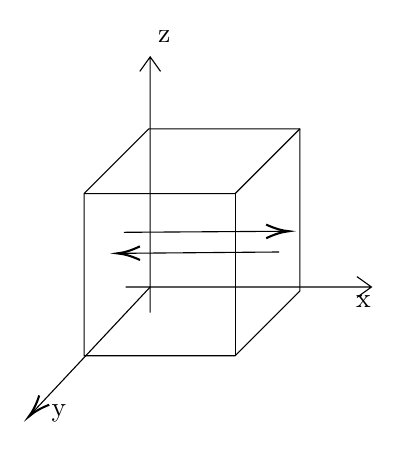
\begin{tikzpicture}[x=0.75pt,y=0.75pt,yscale=-1,xscale=1]
    %uncomment if require: \path (0,444); %set diagram left start at 0, and has height of 444
    
    %Shape: Cube [id:dp9744610415222505] 
    \draw   (234.2,108.34) -- (265.4,77.14) -- (338.2,77.14) -- (338.2,155.28) -- (307,186.48) -- (234.2,186.48) -- cycle ; \draw   (338.2,77.14) -- (307,108.34) -- (234.2,108.34) ; \draw   (307,108.34) -- (307,186.48) ;
    %Shape: Axis 2D [id:dp0363581459664335] 
    \draw  (254.2,153.35) -- (372.67,153.35)(266.05,42.48) -- (266.05,165.67) (365.67,148.35) -- (372.67,153.35) -- (365.67,158.35) (261.05,49.48) -- (266.05,42.48) -- (271.05,49.48)  ;
    %Straight Lines [id:da48208874991326023] 
    \draw    (266.05,153.35) -- (208.9,214.35) ;
    \draw [shift={(207.53,215.81)}, rotate = 313.13] [color={rgb, 255:red, 0; green, 0; blue, 0 }  ][line width=0.75]    (10.93,-3.29) .. controls (6.95,-1.4) and (3.31,-0.3) .. (0,0) .. controls (3.31,0.3) and (6.95,1.4) .. (10.93,3.29)   ;
    %Straight Lines [id:da3905546748423083] 
    \draw    (253.33,127) -- (330.87,126.49) ;
    \draw [shift={(332.87,126.48)}, rotate = 179.62] [color={rgb, 255:red, 0; green, 0; blue, 0 }  ][line width=0.75]    (10.93,-3.29) .. controls (6.95,-1.4) and (3.31,-0.3) .. (0,0) .. controls (3.31,0.3) and (6.95,1.4) .. (10.93,3.29)   ;
    %Straight Lines [id:da40780382647897895] 
    \draw    (328.2,136.48) -- (252.2,137.12) ;
    \draw [shift={(250.2,137.14)}, rotate = 359.51] [color={rgb, 255:red, 0; green, 0; blue, 0 }  ][line width=0.75]    (10.93,-3.29) .. controls (6.95,-1.4) and (3.31,-0.3) .. (0,0) .. controls (3.31,0.3) and (6.95,1.4) .. (10.93,3.29)   ;
    
    
    % Text Node
    \draw (364,156.33) node [anchor=north west][inner sep=0.75pt]   [align=left] {x};
    % Text Node
    \draw (217.33,208.67) node [anchor=north west][inner sep=0.75pt]   [align=left] {y};
    % Text Node
    \draw (268.67,28.67) node [anchor=north west][inner sep=0.75pt]   [align=left] {z};
    
    
    \end{tikzpicture} 
\end{center}
考虑到x方向上的碰撞,我们根据压强的定义:
\begin{align*}
    &P=\frac{F}{S}\\
    &F=\frac{\Delta p}{\Delta t}=\frac{2mv_x}{2x/v_x}=\frac{mv_x^2}{x}\\
    &P=\sum_i \frac{mv_{ix}^2}{xyz}=\frac{m\overline{v^2} N}{3V}=\frac{2}{3}n\overline{\varepsilon} 
\end{align*}
由上述两个不同的压强公式得到:
\begin{align*}
    \frac{2}{3}\overline{\varepsilon}=kT\\
    \overline{\varepsilon} = \frac{3}{2}kT
\end{align*}
这就是所谓的能量均分定理,在这个问题当中平均平动能由三个自由度.自由度受约束的影响,
如果没有约束考虑到3N个自由度,如果由l个约束,则自由度变成3N-l个。
\subsection{麦克斯韦速度分布}
麦克斯韦速率分布函数:
\begin{align*}
    f(v)=4\pi (\frac{m_0}{2\pi kT})^{\frac{3}{2}}\exp(-\frac{m_0 v_x^2}{2kT})v^2
\end{align*}
推导:对于速度来说是一个矢量可以分解为x,y,z三个方向,此时的$f(v)dv\propto \exp(\frac{1}{2}m_v^2/kT)dv$,
对应于v空间上的一个轴上速度在$v_x-v_x+dv_x$的分子数,如果现在扩展到速率的话是一个标量
对应于一层球壳,体积为:$4\pi v^2 dv$,则在这层球壳中的分子数为$\exp(\frac{1}{2}mv^2/kT)v^2dv$,对
这两个积分进行归一化就得到了速率分布函数和速度分布函数。(高斯积分的应用)
\begin{center}
    \begin{tikzpicture}
        \begin{axis}[
            title=在不同温度下的速率分布曲线,
            xmin=0,ymin=0,
            ymax=1.5,
            xlabel={$v$},
            ylabel={$f(v)$},
            samples=201,
            % axis lines=left,
        ]
        \addplot[color=blue,very thick]{4*pi*(1/(0.4*pi))^1.5*x^2*exp(-x^2/0.4)};
        \addplot[color=green,very thick]{4*pi*(1/(pi))^1.5*x^2*exp(-x^2)};
        \addplot[color=orange,very thick]{4*pi*(1/(2*pi))^1.5*x^2*exp(-x^2/2)};
    \end{axis}
    \end{tikzpicture} 
\end{center}
麦克斯韦速率分布函数的物理意义:
\begin{align*}
    \frac{dN/N}{dv}=f(v)\\
    \int_{0}^{\infty}f(v)dv=\int_{0}^{\infty}\frac{dN}{N}=1
\end{align*}
我们到现在为止一共得到了三种速率:
\begin{align*}
    &\overline{v}=\int_{0}^{\infty} vf(v)dv=\sqrt{\frac{8RT}{\pi M}}\\
    &\overline{v^2}=\int_0^\infty v^2f(v)dv=\sqrt{\frac{3RT}{M}}\\
    &v_p=\frac{df(v)}{dv}=\sqrt{\frac{2RT}{M}}
\end{align*}
第一个速率被称为平均速率,可以用来代表分子运动的平均速率,第二个被称为方均根速率,可以使用在分子的
平均平动能中使用,第三个代表的是那个区间的速率分布是最多的。

\subsection{平均自由程}
根据上诉对三个速率的推导,我们可以知道在求分子运动的平均自由程时,我们使用平均速率。
实际上的分子之间也是有碰撞的,根据碰撞的距离和频率,我们得到平均自由程的定义:
\begin{center}
    

\tikzset{every picture/.style={line width=0.75pt}} %set default line width to 0.75pt        

\begin{tikzpicture}[x=0.75pt,y=0.75pt,yscale=-1,xscale=1]
%uncomment if require: \path (0,300); %set diagram left start at 0, and has height of 300

%Shape: Rectangle [id:dp8460867324743337] 
\draw   (149.72,206.93) -- (322.43,121.35) -- (334.14,144.97) -- (161.43,230.55) -- cycle ;
%Shape: Circle [id:dp5038723321764256] 
\draw   (298.17,132.01) .. controls (295.23,125.31) and (298.27,117.49) .. (304.97,114.55) .. controls (311.67,111.61) and (319.49,114.65) .. (322.43,121.35) .. controls (325.38,128.05) and (322.33,135.87) .. (315.63,138.81) .. controls (308.93,141.75) and (301.12,138.71) .. (298.17,132.01) -- cycle ;
%Straight Lines [id:da0548315450682364] 
\draw  [dash pattern={on 4.5pt off 4.5pt}]  (155.93,219.08) -- (327.93,132.83) ;
%Shape: Circle [id:dp17776329976382765] 
\draw   (159.45,216.58) .. controls (156.51,209.88) and (159.55,202.06) .. (166.25,199.12) .. controls (172.95,196.18) and (180.77,199.22) .. (183.71,205.92) .. controls (186.66,212.62) and (183.61,220.44) .. (176.91,223.38) .. controls (170.21,226.32) and (162.4,223.28) .. (159.45,216.58) -- cycle ;

%Straight Lines [id:da5218264082855522] 
\draw    (185.93,57.49) -- (267,108.87) ;
%Straight Lines [id:da7069655461775521] 
\draw    (267,108.87) -- (311.67,52.2) ;
%Straight Lines [id:da18796086379000632] 
\draw    (185.93,57.49) -- (125.67,103.53) ;
%Straight Lines [id:da19092747011263156] 
\draw    (311.67,52.2) -- (389,100.2) ;
%Straight Lines [id:da6361590186824795] 
\draw    (389,100.2) -- (427.67,52.2) ;

%Straight Lines [id:da1094948196815253] 
\draw    (152.67,90) -- (177.73,169.63) ;
\draw [shift={(178.33,171.53)}, rotate = 252.53] [color={rgb, 255:red, 0; green, 0; blue, 0 }  ][line width=0.75]    (10.93,-3.29) .. controls (6.95,-1.4) and (3.31,-0.3) .. (0,0) .. controls (3.31,0.3) and (6.95,1.4) .. (10.93,3.29)   ;
%Shape: Circle [id:dp6836191081123892] 
\draw   (173.1,57.49) .. controls (173.1,50.41) and (178.84,44.66) .. (185.93,44.66) .. controls (193.02,44.66) and (198.76,50.41) .. (198.76,57.49) .. controls (198.76,64.58) and (193.02,70.33) .. (185.93,70.33) .. controls (178.84,70.33) and (173.1,64.58) .. (173.1,57.49) -- cycle ;
%Shape: Circle [id:dp811349450004301] 
\draw   (254.17,108.87) .. controls (254.17,101.78) and (259.91,96.03) .. (267,96.03) .. controls (274.09,96.03) and (279.83,101.78) .. (279.83,108.87) .. controls (279.83,115.95) and (274.09,121.7) .. (267,121.7) .. controls (259.91,121.7) and (254.17,115.95) .. (254.17,108.87) -- cycle ;
%Shape: Circle [id:dp5873365359997111] 
\draw   (298.83,52.2) .. controls (298.83,45.11) and (304.58,39.37) .. (311.67,39.37) .. controls (318.75,39.37) and (324.5,45.11) .. (324.5,52.2) .. controls (324.5,59.29) and (318.75,65.03) .. (311.67,65.03) .. controls (304.58,65.03) and (298.83,59.29) .. (298.83,52.2) -- cycle ;
%Shape: Circle [id:dp5975496475986706] 
\draw   (376.17,100.2) .. controls (376.17,93.11) and (381.91,87.37) .. (389,87.37) .. controls (396.09,87.37) and (401.83,93.11) .. (401.83,100.2) .. controls (401.83,107.29) and (396.09,113.03) .. (389,113.03) .. controls (381.91,113.03) and (376.17,107.29) .. (376.17,100.2) -- cycle ;
%Shape: Circle [id:dp5511166470665791] 
\draw   (414.83,52.2) .. controls (414.83,45.11) and (420.58,39.37) .. (427.67,39.37) .. controls (434.75,39.37) and (440.5,45.11) .. (440.5,52.2) .. controls (440.5,59.29) and (434.75,65.03) .. (427.67,65.03) .. controls (420.58,65.03) and (414.83,59.29) .. (414.83,52.2) -- cycle ;


% Text Node
\draw (240.67,188.33) node [anchor=north west][inner sep=0.75pt]   [align=left] {平均自由程$\displaystyle \lambda =\frac{\overline{v} t}{5}$};
% Text Node
\draw (362,147.33) node [anchor=north west][inner sep=0.75pt]   [align=left] {频率=5};


\end{tikzpicture}
\end{center}
平均自由程定义:
\begin{align*}
    \overline{\lambda}=\frac{\overline{v}}{\overline{Z}}=\frac{1}{\sqrt{2}\pi d^2n}
\end{align*}
气体的密度一定时,分子的有效直径随温度的升高而减小。
\subsection{热力学三定律框架}
热力学的结论都是由这热力学三定律展开的,在这里给一个概览:热力学第零定律引出了温度的
概念,热一引入了能量守恒定律,内能,卡诺循环,卡诺热机,可逆过程,制冷剂,热二引入了熵,
玻尔兹曼关系,熵增原理。接下来将具体论述这些过程。
\subsection{热力学第0定律}
当两个物体分别与第三个物体平衡,那么这两个物体也是处于热平衡,处于热平衡的两个
物体的温度相同
\subsection{热力学第一定律}
能量守恒定律:
\begin{align*}
    \Delta U = \Delta Q +\Delta W
\end{align*}
文字描述:系统的内能的变化有两个方式,一是外界提供给系统的热能,二是外界对系统
做的功。

其中$\Delta W = -\int_1^2 pdV$,这个式子仅对可逆过程成立。对于不可逆过程
还有摩擦力做功或者太快的压缩使得产生冲击波,这些不可逆过程都会产生额外
的功,因此对于不可逆过程:$\Delta W \geq -\int_1 ^2 pdV$。

只有准静态过程可以使用P-V图来表示,并且做功不只与始末位置有关还与中间过程有关。
第一类永动机:不需要为它提供能量也可以为外界做功。这是违反热力学第一定律的。

热容:单位温度所能容纳的热量,等体过程:引入定容摩尔热容:
\begin{align*}
    &A=0\\
    &dU=\frac{m}{M}C_{v,m}dT
\end{align*}

等压过程:引入定压摩尔热容:
\begin{align*}
    &PdV=\mu R dT\\
    &dU=dQ-PdV\\
    &C_{p,m}-C_{v,m}=R
\end{align*}

等温过程:内能只与温度和分子热运动有关$dU=\mu C_{v,m} dT$,因此:
\begin{align*}
    &PV=\mu RT,\Delta U=0\\
    &\Delta Q = -A=\int_1^2 \frac{\mu RT}{V}dV=\mu RT\ln \frac{V_2}{V_1}    
\end{align*}

绝热过程:系统与外界无热量交换:
\begin{align*}
    &\Delta Q=0\\
    &\Delta U=A \Rightarrow A = \mu C_{v,m}\Delta T\\
    &-pdV = \mu C_{v,m} dT\Rightarrow -\frac{\mu R T}{V}dV = \mu C_{v,m}dT\\
    &\ln \frac{V_2}{V_1}=-\frac{C_{v,m}}{R}\ln \frac{T_2}{T_1}  \\
\end{align*}
采用分离变量法:
\begin{align*}
    &C_{p,m}-C_{v,m}=R,\gamma = \frac{C_{p,m}}{C_{v,m}}\\
    &\frac{V_2^{1-\gamma}}{T_2}=\frac{V_1^{1-\gamma}}{T_1}=C\\
    &TV^{\gamma -1}=C
\end{align*}
又因为:$PV \propto T$:
\begin{align*}
    PV^{\gamma-1}=C  
\end{align*}
卡诺热机由四个过程组成:等温膨胀,绝热膨胀,等温压缩,绝热压缩。可以根据此推导出
温度和Q的关系,以及卡诺热机的效率。
\begin{align*}
    \begin{cases}
        T_1V_1^{\gamma-1}=T_2V_3^{\gamma-1}\\
        T_1V_1^{\gamma-1}=T_2V_4^{\gamma-1}
    \end{cases}
    \Rightarrow \frac{V_4}{V_3}=\frac{V_1}{V_2}
\end{align*}
$T_1$表示高温热源,$T_2$表示低温热源
\begin{align*}
    &Q_1=\mu RT_1\ln\frac{V_2}{V_1}\\
    &Q_2=- \mu RT_2\ln\frac{V_3}{V_4}\\
    &\frac{Q_1}{Q_2}=-\frac{T_1}{T_2}\\
    &\eta =\frac{Q_1+Q_2}{Q_1} =1-\frac{T_2}{T_1}
\end{align*}

制冷机:外界对系统做功使得热量从低温物体转移到高温物体。卡诺热机是可逆热机。
制冷机的效率:$$\eta=\frac{Q_2}{A}=\frac{Q_2}{Q_1+ Q_2}=\frac{T_2}{T_1-T_2}$$
,制冷机的效率大于$100\%$。

还有热泵(heat pump)其实是另外一种制冷机,相当于室内暖气的工作原理,制冷机我们需要的是它的
热量,而不是功,因此效率为:
\begin{align*}
    \eta = \frac{Q_1}{A}=\frac{Q_1}{Q_1+Q_2}=\frac{T_2}{T_2-T_1}
\end{align*}
此时的效率还是大于100\%
\subsection{热力学第二定律}
两种表述:1. 开尔文表述:不可能从单一热源吸收热量使之完全变成有用功而不产生其他
影响。2. 克劳修斯表述:热量不可能自发地从低温物体传到高温物体。

证明两种表述的一致性:考虑到两个热机工作在高温热源和低温热源之间。假设有两个卡诺热机
其中一个热机从高温热源吸收热量使之完全变成有用功,完全的有用功使得另外一个热机从低温
热源吸收热量$Q_1$,然后向高温热源释放$Q_1+Q_2$的热量,总体上来看这个热机,在没有外界
的作用下,竟然能自发的从低温热源吸收热量$Q_1$向高温热源释放热量。因此这两种表述是等价的.
\begin{center}
    

\tikzset{every picture/.style={line width=0.75pt}} %set default line width to 0.75pt        

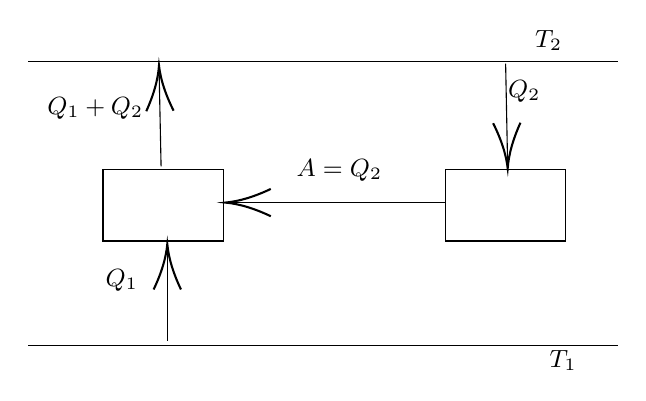
\begin{tikzpicture}[x=1.5pt,y=1.5pt,yscale=-1,xscale=1]
%uncomment if require: \path (0,300); %set diagram left start at 0, and has height of 300

%Straight Lines [id:da11754561757066329] 
\draw    (214.1,133.3) -- (356.1,133.3) ;
%Straight Lines [id:da6804186865474866] 
\draw    (214.1,201.8) -- (356.1,201.8) ;
%Shape: Rectangle [id:dp8033049691542808] 
\draw   (314.6,159.3) -- (343.6,159.3) -- (343.6,176.55) -- (314.6,176.55) -- cycle ;
%Shape: Rectangle [id:dp511267409384953] 
\draw   (232.1,159.3) -- (261.1,159.3) -- (261.1,176.55) -- (232.1,176.55) -- cycle ;
%Straight Lines [id:da9254637526684772] 
\draw    (329.1,133.8) -- (329.56,157.05) ;
\draw [shift={(329.6,159.05)}, rotate = 268.87] [color={rgb, 255:red, 0; green, 0; blue, 0 }  ][line width=0.75]    (10.93,-3.29) .. controls (6.95,-1.4) and (3.31,-0.3) .. (0,0) .. controls (3.31,0.3) and (6.95,1.4) .. (10.93,3.29)   ;
%Straight Lines [id:da8663621785827107] 
\draw    (314.6,167.3) -- (263.6,167.3) ;
\draw [shift={(261.6,167.3)}, rotate = 360] [color={rgb, 255:red, 0; green, 0; blue, 0 }  ][line width=0.75]    (10.93,-3.29) .. controls (6.95,-1.4) and (3.31,-0.3) .. (0,0) .. controls (3.31,0.3) and (6.95,1.4) .. (10.93,3.29)   ;
%Straight Lines [id:da6770363582482] 
\draw    (247.6,200.55) -- (247.6,179.3) ;
\draw [shift={(247.6,177.3)}, rotate = 90] [color={rgb, 255:red, 0; green, 0; blue, 0 }  ][line width=0.75]    (10.93,-3.29) .. controls (6.95,-1.4) and (3.31,-0.3) .. (0,0) .. controls (3.31,0.3) and (6.95,1.4) .. (10.93,3.29)   ;
%Straight Lines [id:da9440357094713592] 
\draw    (246.1,158.55) -- (245.64,136.3) ;
\draw [shift={(245.6,134.3)}, rotate = 88.82] [color={rgb, 255:red, 0; green, 0; blue, 0 }  ][line width=0.75]    (10.93,-3.29) .. controls (6.95,-1.4) and (3.31,-0.3) .. (0,0) .. controls (3.31,0.3) and (6.95,1.4) .. (10.93,3.29)   ;


% Text Node
\draw (335.6,125.3) node [anchor=north west][inner sep=0.75pt]  [font=\fontsize{0.9em}{0.9em}\selectfont] [align=left] {$\displaystyle T_{2}$};
% Text Node
\draw (339.1,202.3) node [anchor=north west][inner sep=0.75pt]  [font=\fontsize{0.9em}{0.9em}\selectfont] [align=left] {$\displaystyle T_{1}$};
% Text Node
\draw (329.1,137.3) node [anchor=north west][inner sep=0.75pt]  [font=\fontsize{0.9em}{0.9em}\selectfont] [align=left] {$\displaystyle Q_{2}$};
% Text Node
\draw (278.1,156.3) node [anchor=north west][inner sep=0.75pt]  [font=\fontsize{0.9em}{0.9em}\selectfont] [align=left] {$\displaystyle A=Q_{2}$};
% Text Node
\draw (232.1,182.8) node [anchor=north west][inner sep=0.75pt]  [font=\fontsize{0.9em}{0.9em}\selectfont] [align=left] {$\displaystyle Q_{1}$};
% Text Node
\draw (218.1,141.3) node [anchor=north west][inner sep=0.75pt]  [font=\fontsize{0.9em}{0.9em}\selectfont] [align=left] {$\displaystyle Q_{1} +Q_{2}$};


\end{tikzpicture}
\end{center}

可逆过程与不可逆过程:可逆过程指的是物体从状态A到B,存在另外一个过程,从B到A,周围
的一切也都恢复原状。

\textbf{卡诺定理:}可逆热机的效率一定是大于或等于不可逆热机的。证明过程类似于热力学第二定律的证明:
如何判断是否是可逆过程,一种方法就是可以使用定义来判断,即是否存在一个与之相反的过程
并且能使外界条件恢复原样。二是直接通过热力学第二定律的两种表述来判断:功通过摩擦转变
为热的过程是不可逆过程,否则违反开尔文表述,热量从高温物体到低温物体是一种不可逆过程
否则违反克劳修斯表述。

\textbf{熵:}由可逆过程引入的一个态函数:
\begin{align*}
    &\sum \frac{Q}{T}=\sum\frac{\Delta Q}{T}=0\Rightarrow \oint \frac{dQ}{T}=0\\
    &\int _1^2 \frac{dQ}{T}=S_2-S_1
\end{align*}
上式中,我们定义了熵变。$\Delta S=\Delta Q/T$只能是可逆过程中熵变的定义,如果
是在不可逆过程当中只能使用熵只与始末位置有关来求,因此我们可以设想任意一个可逆过程
使始末达到的状态与不可逆过程的始末态一样,然后根据可逆过程中熵的定义来求熵变。

\textbf{熵增原理的描述}:对于一孤立系统或者绝热系统中发生的不可逆过程
都会使得熵增加。注意是封闭系统或者绝热系统,否则可以借助外界条件使得熵不增加。

\textbf{热力学第二定律的统计诠释(玻尔兹曼关系):}
\begin{align*}
    S=k\ln \Omega
\end{align*}

例子:气体自由膨胀的不可逆性,设想开始由四个粒子位于A室,0个粒子位于B室,在自由膨胀
之后,会出现以下可能性:
\begin{center}
    \begin{table}[htbp]
        \centering
        \caption{粒子的微观状态数}
        \begin{tabular}{ccccccccccccccccc}
            \toprule  % 顶部线
            A&0&a&b&c&d&ab&
            ac&ad&bc&bd&cd&abc&abd&acd&bcd&abcd \\ 
            \cmidrule{1-17}
            B&abcd&bcd&acd&abd&abc&cd&bd&bc&ad&ac&ab&d&c&b&a&0 \\
            \bottomrule  % 底部线
        \end{tabular}
\end{table}  
\end{center}

开始只有一个微观态,现在有16个微观态,因此微观状态数也从侧面反映出来熵增导致了微观状态数的增加从而
导致无序混乱的增加。
\newpage
\section{电磁学}
\subsection{静电学}
1. 库伦定律:
\begin{align*}
    F=-\frac{1}{4\pi \varepsilon_0}\frac{q_1q_2}{r^2}
\end{align*}

2. 没有接触的物体之间产生相互作用,必须有传递介质,在真空中电磁相互作用仍然存在,这是因为存在电场和磁场作为传递介质,电场和磁场都是
实际存在的物质。只不过是物质存在的一种形式。因此需要引入电场和磁场,电场的定义:
\begin{align*}
    E=\frac{F}{q}=-\frac{1}{4\pi\varepsilon_0}\frac{q}{r^2}
\end{align*}
此时的q是场源电荷,电场能反映出空间的性质,与试探电荷无关。电场是矢量场,电场的
叠加满足叠加原理。

3. 电偶极矩:如果考虑到这样一种情况:左边是一个负电荷,右边是一个正电荷,其电偶极矩的大小:$p=ql$
,方向从负电荷指向正电荷。

4. 电势和电势能:
和一般的势能一样定义,这里的电势能的改变对应于电场力的做功,为了引入一个新的只与电场有关的物理量
,因此定义电势:$U=W_a/q$,两个物理量和电场的关系:
\begin{align*}
    \int _1^2 Eqdl = W_2-W_1\Rightarrow \int_1^2 Edl = U_2-U_1
\end{align*}

5. 静电场是保守场,对于所有的保守场有这样两个性质:
\begin{align*}
    &\oint Eq dl =0\Rightarrow \oint E dl =0\\
    &F=Eq=-\nabla W_a \Rightarrow E=-\nabla U
\end{align*}
电势的叠加原理:由于电势是标量,可以直接进行标量运算,如果需要通过电势计算
电场,只需要对电势作梯度运算即可。

6.静电场中的导体:
因为导体中的自由电子由于电场的作用下会发生移动,这样就会在导体内部产生一个
电场,当这种运动达到平衡时,导体内部的电场和外部电场抵消了,所以电场中的导体有
这样几个性质:(1)导体内部的场强处处为0,(2)整个导体是一个等势体,(3)表面是一个等势面。

7.电容:
\begin{align*}
    C=\frac{Q}{U}
\end{align*}
电容是指容纳电荷的能力,电容器的串联和并联根据定义式来。

8.电介质的极化:在电解质中,有有极分子和无极分子,这两种分子的划分依据是其电偶极矩是否为0,
无极分子的电偶极矩为0,有极分子电偶极矩不为0,当电介质放在电场中,其中的有极分子发生取向极化
,无极分子发生位移极化,总的效果是产生了与外电场方向相反的电场,对比导体内部产生电场的微观机制
,但是电解质产生的这种电场是很小的,根据麦克斯韦方程组的假设,电场产生的源是电荷,可以把极化电场
等效为极化电荷的效果,引入极化强度(单位体积内所有的电偶极矩的总和),接下来是一些数学推导:
\begin{align*}
    P=\frac{\sum p}{V}\Rightarrow \sum p = PSl=q'l\qquad P=\sigma'
\end{align*}
\subsection{静磁学}
1. 电流的定义:
\begin{align*}
    I=\frac{dq}{dt}\Rightarrow dI=JdS
\end{align*}

2.电动势:为了描述电源内部非静电力做功而引入的物理量$\varepsilon=\frac{dA}{dq}$
因为描述的是非静电力,是非保守力,因此环路积分不等于0:$\oint E dl =\varepsilon$,
其中$\varepsilon$表示电动势。

3. 毕奥-萨法尔定律:
\begin{align*}
    dB=\frac{\mu_0}{4\pi}\frac{Idl\times e_r}{r^2}
\end{align*}

4. 磁力:这里的内容是我对格里菲斯电动力学上面讲解的理解,
\begin{align*}
    F=qv\times B
\end{align*}
由于v和F垂直,因此洛伦兹力不做功,洛伦兹力宏观表现为安培力,考虑在一维的电荷
的运动,在单位时间内通过长度为vdt的电荷量等于电流的大小,数学形式:$\lambda  vdt=I$($\lambda$是线电荷)
\begin{align*}
    F= qI/\lambda \times B=Idl\times B
\end{align*}
考虑一个通电线框的运动:
\begin{center}
    

\tikzset{every picture/.style={line width=0.75pt}} %set default line width to 0.75pt        

\begin{tikzpicture}[x=0.75pt,y=0.75pt,yscale=-1,xscale=1]
%uncomment if require: \path (0,300); %set diagram left start at 0, and has height of 300

%Shape: Rectangle [id:dp23090302911769256] 
\draw   (90.54,44.75) -- (227.9,44.75) -- (227.9,116.89) -- (90.54,116.89) -- cycle ;
%Shape: Rectangle [id:dp08965474088205472] 
\draw   (112.91,96.69) -- (199.64,96.69) -- (199.64,138.53) -- (112.91,138.53) -- cycle ;
%Straight Lines [id:da5389780570213296] 
\draw    (154.12,138.89) -- (154.12,168.11) -- (154.12,193.36) ;
%Shape: Rectangle [id:dp9952724435198153] 
\draw   (137.24,193.36) -- (170.6,193.36) -- (170.6,215) -- (137.24,215) -- cycle ;
%Straight Lines [id:da11019032216619684] 
\draw    (112.91,96.69) -- (197.64,96.69) ;
\draw [shift={(199.64,96.69)}, rotate = 180] [color={rgb, 255:red, 0; green, 0; blue, 0 }  ][line width=0.75]    (10.93,-3.29) .. controls (6.95,-1.4) and (3.31,-0.3) .. (0,0) .. controls (3.31,0.3) and (6.95,1.4) .. (10.93,3.29)   ;
\draw   (147.38,89.87) .. controls (151.49,86.14) and (158.09,86.15) .. (162.12,89.9) .. controls (166.15,93.65) and (166.09,99.72) .. (161.98,103.45) .. controls (157.87,107.19) and (151.27,107.17) .. (147.24,103.42) .. controls (143.2,99.67) and (143.27,93.6) .. (147.38,89.87) -- cycle ; \draw   (147.38,89.87) -- (161.98,103.45) ; \draw   (162.12,89.9) -- (147.24,103.42) ;
%Straight Lines [id:da05875874706628492] 
\draw    (156.28,96.69) -- (156.28,20.06) ;
\draw [shift={(156.28,18.06)}, rotate = 90] [color={rgb, 255:red, 0; green, 0; blue, 0 }  ][line width=0.75]    (10.93,-3.29) .. controls (6.95,-1.4) and (3.31,-0.3) .. (0,0) .. controls (3.31,0.3) and (6.95,1.4) .. (10.93,3.29)   ;

%Straight Lines [id:da2689416577997066] 
\draw    (336.3,177.82) -- (538.8,177.82) ;
%Straight Lines [id:da013174381045838679] 
\draw    (437.55,177.82) -- (496.31,127.34) ;
\draw [shift={(497.83,126.03)}, rotate = 139.33] [color={rgb, 255:red, 0; green, 0; blue, 0 }  ][line width=0.75]    (10.93,-3.29) .. controls (6.95,-1.4) and (3.31,-0.3) .. (0,0) .. controls (3.31,0.3) and (6.95,1.4) .. (10.93,3.29)   ;
%Straight Lines [id:da18202667363100167] 
\draw    (496.65,176.05) -- (496.65,136.89) ;
\draw [shift={(496.65,134.89)}, rotate = 90] [color={rgb, 255:red, 0; green, 0; blue, 0 }  ][line width=0.75]    (10.93,-3.29) .. controls (6.95,-1.4) and (3.31,-0.3) .. (0,0) .. controls (3.31,0.3) and (6.95,1.4) .. (10.93,3.29)   ;
%Straight Lines [id:da2750400806239206] 
\draw    (437.55,177.82) -- (503.71,178.25) ;
\draw [shift={(505.71,178.26)}, rotate = 180.37] [color={rgb, 255:red, 0; green, 0; blue, 0 }  ][line width=0.75]    (10.93,-3.29) .. controls (6.95,-1.4) and (3.31,-0.3) .. (0,0) .. controls (3.31,0.3) and (6.95,1.4) .. (10.93,3.29)   ;
%Straight Lines [id:da4420305610848654] 
\draw    (437.55,177.82) -- (437.55,76.69) ;
\draw [shift={(437.55,74.69)}, rotate = 90] [color={rgb, 255:red, 0; green, 0; blue, 0 }  ][line width=0.75]    (10.93,-3.29) .. controls (6.95,-1.4) and (3.31,-0.3) .. (0,0) .. controls (3.31,0.3) and (6.95,1.4) .. (10.93,3.29)   ;
%Straight Lines [id:da8633509773160777] 
\draw    (437.55,177.82) -- (362.06,93.01) ;
\draw [shift={(360.73,91.51)}, rotate = 48.33] [color={rgb, 255:red, 0; green, 0; blue, 0 }  ][line width=0.75]    (10.93,-3.29) .. controls (6.95,-1.4) and (3.31,-0.3) .. (0,0) .. controls (3.31,0.3) and (6.95,1.4) .. (10.93,3.29)   ;
%Straight Lines [id:da9610403003945396] 
\draw  [dash pattern={on 4.5pt off 4.5pt}]  (360.73,91.51) -- (360.73,177.38) ;


% Text Node
\draw (347.35,79.53) node [anchor=north west][inner sep=0.75pt]   [align=left] {$\displaystyle F$};
% Text Node
\draw (426.58,52.97) node [anchor=north west][inner sep=0.75pt]   [align=left] {$\displaystyle F_{a}$};
% Text Node
\draw (494.5,103.43) node [anchor=north west][inner sep=0.75pt]   [align=left] {$\displaystyle v$};
% Text Node
\draw (460.02,181.33) node [anchor=north west][inner sep=0.75pt]   [align=left] {$\displaystyle u$};
% Text Node
\draw (512.89,144.15) node [anchor=north west][inner sep=0.75pt]   [align=left] {$\displaystyle w$};


\end{tikzpicture}
\end{center}
导线当中的带电粒子的运动并不是竖直方向上的,而是指向右上方的,因此可以考虑两个
方向上的运动,先考虑竖直方向上的,正好就是安培力做功,水平方向上会有一个阻碍
电荷流动的力,但是实际上并没有阻碍电流的力,因为此时电源对电荷做功克服了这个力,
从整个过程的角度来思考:磁力(洛伦兹力)并没有做功,它起到了一个媒介的作用,安培力
做功从根源上来看还是电源做功转化而来的。

5. 顺磁,抗磁,铁磁性与磁化的概念

抗磁性:自身的总磁矩为0,但是会有进动现象,导致产生附加磁矩,这个附加磁矩方向和原本
的磁场方向相反。导致总的磁场相对于原本的磁场减弱。

顺磁性:分子磁矩需要保持能量最低的状态,平衡时遵循玻尔兹曼分布,自身产生的磁矩远大于进动
产生的附加磁矩,使得最后的总的磁场方向相对于原本的磁场方向增强(抗磁性是普遍存在的)

铁磁性:铁磁性物质,磁化曲线不是线性的。存在一个温度临界点(居里温度),在达到
该温度后磁性发生突变,变成顺磁质。

上面几种现象不管是和原磁场是抵消还是加强都成为磁化。

磁化的概念:类比电偶极矩$M = p\times E$,磁矩:$M=p_m \times B$(其中$p_m=IS\vec{n}$),
根据安培的分子电流假设,每个磁矩都可以使用分子电流来代替,假设是均匀介质,内部电流互相抵消了
,只有外部电流,考虑到抗磁性是每中介质当中都有的,表现顺磁性的介质对磁场的影响
远大于抗磁性对磁场的影响,磁化电流(束缚电流)产生的B'是对B加强的,可以使用如上分析
得到在磁介质影响下的安培环路定律,数学推导(M表示单位长度的电流):
\begin{align*}
    \mathbf{M}=\frac{\sum m}{V}\Rightarrow \sum m = MlS=I'S
\end{align*}


理解H和B的关系,H是实际磁场的大小,而B是粒子对H感应的磁场大小,从洛伦兹力公式和安培力公式
就可以看出来,当介质是表现为顺磁性和抗磁性时B和H为线性关系,无法体现出这种关系,但是介质为铁磁物质的时候,这种
感应关系就很明显了,具体可以通过磁滞回线表现出:
\begin{center}
    

\tikzset{every picture/.style={line width=0.75pt}} %set default line width to 0.75pt        

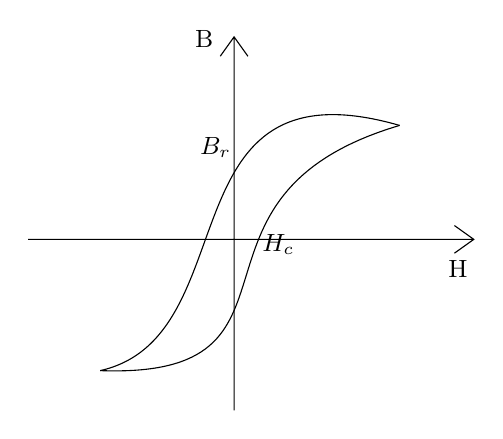
\begin{tikzpicture}[x=1pt,y=1pt,yscale=-1,xscale=1]
%uncomment if require: \path (0,300); %set diagram left start at 0, and has height of 300

%Shape: Axis 2D [id:dp7065972720973936] 
\draw  (281.84,158.09) -- (442.84,158.09)(356.22,84.92) -- (356.22,219.92) (435.84,153.09) -- (442.84,158.09) -- (435.84,163.09) (351.22,91.92) -- (356.22,84.92) -- (361.22,91.92)  ;
%Curve Lines [id:da4715096999095527] 
\draw    (307.84,205.52) .. controls (390.04,208.52) and (329.64,142.52) .. (416.04,116.92) ;
%Curve Lines [id:da5941739474892351] 
\draw    (307.84,205.52) .. controls (362.04,193.32) and (329.8,92.07) .. (416.04,116.92) ;


% Text Node
\draw (341.2,81.8) node [anchor=north west][inner sep=0.75pt]  [font=\small] [align=left] {B};
% Text Node
\draw (432.7,164.8) node [anchor=north west][inner sep=0.75pt]  [font=\small] [align=left] {H};
% Text Node
\draw (343,120.3) node [anchor=north west][inner sep=0.75pt]  [font=\small] [align=left] {$\displaystyle B_{r}$};
% Text Node
\draw (365.5,155.3) node [anchor=north west][inner sep=0.75pt]  [font=\small] [align=left] {$\displaystyle H_{c}$};


\end{tikzpicture}
\end{center}
当$H=0$时,$B\neq0$,磁感应强度的变化总是落后于磁场强度的变化。当$B=0$时,$H\neq0$
,这个H被称为材料的矫顽力。

\subsection{电动力学}
1. 电磁感应现象的描述:指的是变化的磁场产生的电场,这里的电场能够产生电动势,将
电动势接入闭合回路中将会产生电流,因此,总体上来说,变化的磁场产生感应电流
的现象就叫做电磁感应现象。使用数学化的方法来描述这种现象(法拉第电磁感应定律):
\begin{align*}
    \varepsilon=-N\frac{d\Phi}{dt}\qquad \Phi = BS
\end{align*}
因此B或者S随时间变化就能产生感应电动势。B变化会在周围激发感生电场,感生电场力
提供了感生电动势的非静电力,S变化会使导线做切割磁感线运动,此时洛伦兹力提供
动生电动势的非静电力。数学描述:
\begin{align*}
    \varepsilon = \int E_r dl\qquad\varepsilon = \int v\times B dl 
\end{align*}

2. 自感现象:由于回路自身电流,回路面积等变化引起了磁通量的变化从而产生感应电动势的
现象叫做自感现象。
通电螺线管的自感现象:长l($l>>r$)通电螺线管内部磁场可以使用安培环路定理来求:
\begin{align*}
    \oint B dl = \mu_0 N I \Rightarrow \int B dl =\mu_0 N I\Rightarrow B=\frac{\mu_0NI}{l}
\end{align*}
根据法拉第电磁感应定律:
\begin{align*}
    \varepsilon=-\pi r^2 \frac{\mu_0 N^2}{l}\frac{dI}{dt}=-L\frac{dI}{dt}(L=\frac{\mu_0N^2\pi r^2 }{l})
\end{align*}
L被称为自感系数(一种电磁惯性)。自感系数另外一个定义:
\begin{align*}
    \mathcal{E}=-\frac{d\Phi}{dt}=-\frac{d\Phi}{dI}\frac{dI}{dt}\Rightarrow L=\frac{d\Phi}{dI}
\end{align*}
当L是常数时,$\Psi =N\varPhi = LI$

3. 互感现象:定义类似于自感现象,
匝数为$N_1,N_2$的线圈交叉的缠绕在螺线管上,其中匝数为$N_1$的通电,另外一砸不通电,则
\begin{align*}
    \varepsilon=-\frac{\mu_0 N_1N_2 \pi r^2}{l}\frac{dI}{dt}(M=\frac{\mu_0 N_1N_2 \pi r^2}{l})
\end{align*}
M称为互感系数。观察两种系数的特点,M和L都与电流无关,并且两个系数满足:
\begin{align*}
    M=\sqrt{L_1L_2}
\end{align*}
\subsection{麦克斯韦方程组}
1. 静电荷激发的电场满足高斯定理:
\begin{align*}
    \oiint E dS =\frac{q}{\varepsilon_0} 
\end{align*}
所以对于对称性很高的物体周围的电场可以使用此方法来求,静电场是保守场,激发的电场是保守场
满足环路积分等于0($\oint E dl =0$)

当存在介质时,我们引入极化电荷$q'$,总的电场的高斯定理:
\begin{align*}
    &\oiint E dS = \frac{q}{\varepsilon_0}-\frac{q'}{\varepsilon_0}\\
    &\oiint D dS = q\Rightarrow D=\varepsilon_0 E+P
\end{align*}
由$P=\chi\varepsilon_0 E$得到E和D的关系,这里的E表示的总的电场:
\begin{align*}
    D = \varepsilon_0(1+\chi)E\Rightarrow \varepsilon_r=1+\chi\qquad \varepsilon=\varepsilon_0\varepsilon_r
\end{align*}

2. 由电流激发的磁感应强度B满足安培环路定理:
\begin{align*}
    \oint B dl =\mu_0 I
\end{align*}
磁场是非保守场,磁感应线总是闭合的曲线,其通量总是等于0:($\oiint B dS = 0$)

存在磁介质时,总的磁场B的安培环路定理:
\begin{align*}
    &\oint B dl = \mu_0 I +\mu_0 I'\\
    &\oint H dl = I\Rightarrow H=\frac{B}{\mu_0}-M
\end{align*}
由$M=\chi H$得到B和H的关系:
\begin{align*}
    B=\mu_0(1+\chi)H=\mu H=\mu_0\mu_r H
\end{align*}

3. 引入电磁感应当中的变化的磁场产生电场,这里的电场不再是保守场。
\begin{align*}
    \varepsilon=-\frac{d\Phi}{dt}=\oint E' dl = -S\frac{\partial B}{\partial t}=-\iint \pdv{B}{t} dS
\end{align*}
总的电场等于感生电场加上静电场:
\begin{align*}
    \oint E dl = \oint (E_0+E') dl =0+ -\iint \pdv{B}{t} dS
\end{align*}

4. 当环路中存在电容器时,在电容器这一部分的电流间断了,但是电荷量还是会发生变化。
\begin{align*}
     \oiint D dS = q\Rightarrow D = \sigma
\end{align*}
$\sigma$是极板上的电荷密度,根据电流的定义:
\begin{align*}
    I =\frac{dq}{dt}=S\frac{d\sigma}{dt}=S\frac{dD}{dt}
\end{align*}
因此加上这个等效的电流,整个回路积分就是连续的了,$D=\varepsilon E$
\begin{align*}
    \oint H dl = I+\iint \pdv{D}{t}dS=I+\varepsilon\iint  \pdv{E}{t}dS
\end{align*}
这里的等效电流我们称之为位移电流。这里体现了方程的对称性,右边第二项,可以将其
视为变化的电场产生磁场,这样使得法拉第电磁感应定律更加完备,电场和磁场可以互相激发
。

5. 麦克斯韦方程组的积分形式总结:
\begin{align*}
    &\oiint D dS = q\\
    &\oint E dl = -\iint \pdv{B}{t} dS\\
    &\oint H dl = I+\iint \pdv{D}{t}dS\\
    &\oiint B dS = 0
\end{align*}
由散度定理和旋度定理可以得到:
\begin{align*}
    &\oiint D dS = \iiint \nabla\cdot D dV = \iiint \rho dV\\
    &\oint E dl =\iint \nabla \times E dS= -\iint \pdv{B}{t} dS\\
    &\oint H dl = \iint \nabla \times H dl =\iint j dS+\iint \pdv{D}{t}dS\\
    &\oiint B dS =\iiint \nabla \cdot B =0
\end{align*}
微分形式的麦克斯韦方程组:
\begin{align*}
    &\nabla\cdot D  =  \rho \\
    &\nabla \times E =  -\pdv{B}{t} \\
    &\nabla \times H  = j + \pdv{D}{t}\\
    &\nabla \cdot B =0
\end{align*}
除了关于电磁场的方程,这里还补充三个很重要的方程:
\begin{align*}
    &F=q(E+v\times B)\\
    &\pdv{\rho}{t}=-\nabla \cdot j\\
    &j=\sigma E
\end{align*}
第三个方程就是欧姆定律,电流与每单位电荷所受的力有关($\sigma$就是我们所熟知的电导率,假设这里的v是远小于c的。)
\subsection{电磁场的能量}
1. 电场的能量:电场的能量转化为电荷做功
\begin{align*}
    &dA=Udq=\frac{Q}{C}dq\Rightarrow A=\frac{1}{2C}Q^2
\end{align*}
对于平行板电容器:$W=\int \frac{1 }{2}DEdV$,在其他情况下也是适用的。

2. 磁场的能量:当刚启动电路时,磁场的能量转化为自感产生的能量
\begin{align*}
    &\varepsilon-L\frac{dI}{dt}=IR\\
    &\int \varepsilon Idt -\int LIdI=\int I^2R dt\\
    &\int \varepsilon dq=\frac{1}{2}LI^2+I^2Rt
\end{align*}
在通电螺线管中: $W=\int \frac{1}{2}HBdV$,在其他情况下也是适用的。因此电磁场的总能量
和能量密度可以写为:
\begin{align*}
    W= \iiint(E\cdot D +H\cdot B)  dV\qquad w= E\cdot D+H\cdot B
\end{align*}


\section{机械振动和机械波}
\section{光的波动理论和电磁理论}
\end{document}

